\begin{flushright} {\tiny {\color{gray} strainweakening.tex}} \end{flushright}

Several mechanisms may contribute to strain or strain
rate dependent weakening but their relative and absolute
importance is poorly constrained. Furthermore, 
weakening mechanisms are often crudely parameterised in 
geodynamical codes with simple mathematical functions 
and a limited number of parameters. 

For example, in \cite{alht11} the authors use a von Mises plasticity formulation so that the 
rheology is parameterised by the cohesion $c$, or $c=\sigma_y$ in their notations. The
yield strength $\sigma_y$ starts is constant until the strain
$\varepsilon$ reaches the threshold value $\varepsilon_1$. It then decreases linearly
from $\sigma_y$ to $\sigma_{y}^{sw}$ between $\varepsilon_1$ and $\varepsilon_2$. 
For strain values $\varepsilon>\varepsilon_2$ , the yield strength remains constant 
at $\sigma_y^{sw}$ .

\begin{center}
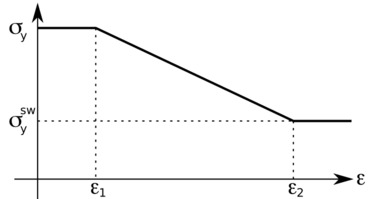
\includegraphics[width=6cm]{images/strainweakening/alht11}\\
{\tiny Taken from \cite{alht11}}
\end{center}

The same authors in a subsequent study use a Drucker-Prager rheology parameterised by 
cohesion $c$ and friction angle $\phi$. They use the same approach as before but now 
both parameters are subjected to strain weakening: 

\begin{center}
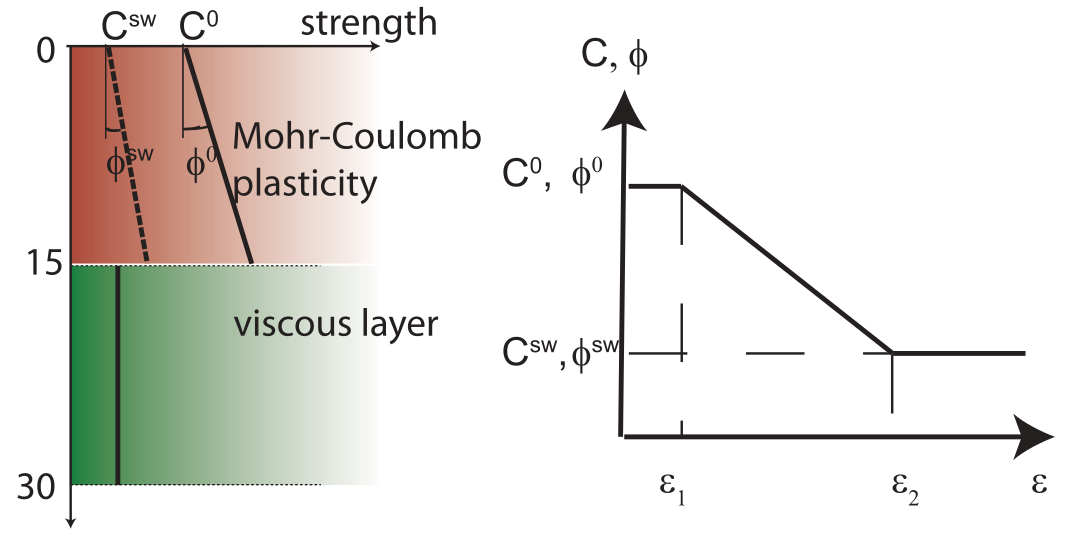
\includegraphics[width=6cm]{images/strainweakening/alht12}\\
{\tiny Taken from \cite{alht12}, see also \cite{thie11}}
\end{center}

They further define the factor $R=C^0/C^{sw}=\phi^0/\phi^{sw}\geq 1$ which is a proxy
for the ratio $\sigma_y/\sigma_y^{sw}$ where $\sigma_y=p \sin\phi + c \; \cos \phi$, 
and carry out 3D crustal extensional models for $R$ between 2 and 5. 


\begin{itemize}
\item In \cite{lemh17} the authors also define 
\[
\tau_y = p \sin (\phi(\varepsilon^p))  + c_0 \cos(\phi(\varepsilon^p))
\]
but the cohesion is regarded to be constant. 
The angle of friction $\phi$ is assumed to decrease as a function of the accumulated plastic
strain $\varepsilon^p$ to
\[
\phi(\varepsilon^p) 
=
\max \left(
\phi_\infty , \phi_0 - \frac{\varepsilon^p (\phi_0-\phi_\infty)}{\varepsilon^p_\infty}
\right)
\]
This equation defines an empirical softening relation which reduces the
friction angle linearly with accumulated plastic strain.
$\phi_0$ defines the initial friction angle, $\varepsilon^p_\infty$
represents the measure of plastic strain after which complete softening is achieved and internal
friction angle reaches $\phi_\infty$ . Plastic strain represents an integrated,
tensorial invariant measure of the deformation which has occurred
due to plastic yielding. Thus, the quantity $\varepsilon^p$ can be regarded as
a simplified measure of material damage. 


\item In Dyksterhuis \etal \cite{dyrm07} a variant of the above formulation is used:
\[
f(\varepsilon)=
\left\{
\begin{array}{cc} 
1-(1-a)(\varepsilon/\varepsilon_0)^n & \varepsilon \leq \varepsilon_0 \\
a &  \varepsilon \geq \varepsilon_0 
\end{array}
\right.
\]
where $\varepsilon$ is the accumulated plastic strain, $\varepsilon_0$ is the
saturation strain beyond which no further weakening
takes place, $n$ is an exponent that controls the shape
of the function and $a$ is a maximum value of strain
weakening beyond which no further weakening
occurs. This equation leads to the following plot:

\begin{center}
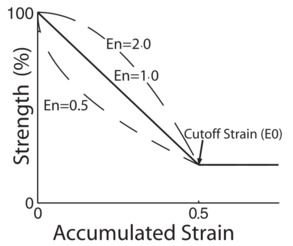
\includegraphics[width=6cm]{images/strainweakening/dyrm07}\\
{\tiny Strain-softening behaviour showing strength weakening from 100 to 20\% 
after an accumulated strain of 0.5, after which no further weakening occurs. 
Dashed lines show the effect of the exponential parameter
(En) on the curve. Taken from \cite{dyrm07}}
\end{center}

Although it is not specified in \cite{dyrm07} what $f$ is, other users of the code 
specify that the yield strength is given by 
\[
\sigma_y = (B_0 + B_1 p ) f(\varepsilon)
\]
where $p$ is the pressure, $B_0$ is the cohesion, or yield stress at
zero pressure, and $B_p$ is the pressure dependence of the yield
stress, equivalent to the friction coefficient in Byerlee's law. 

In \cite{yamz18} the authors take a different approach:
\[
C=C_0+C_1 \exp \left( -\frac{\varepsilon_{plast}}{\varepsilon_{ref}} \right)
\]
\[
\mu=\mu_0+\mu_1 \exp \left( -\frac{\varepsilon_{plast}}{\varepsilon_{ref}} \right)
\]
where $C_0$ and $C_0+C_1$ represent the minimum and maximum cohesions, respectively;
$\mu_0$ and $\mu_0+\mu_1$ represent the minimum and maximum frictional coefficients, respectively. 
$\varepsilon_{plast}$ and $\varepsilon_{ref}$ represent accumulated plastic strain and 
reference strain, respectively.

\index{general}{Plastic Hardening}
\item In \cite{leor89} the authors describe another formulation for plastic hardening. The angle of friction 
changes with the accumulated plastic strain:
\[
\sin \phi = \sin \phi_i  + \frac{2(\sin \phi_f - \sin\phi_i)\sqrt{\varepsilon^p_c  \varepsilon^p }}{\varepsilon^p + \varepsilon^p_c}
\] 
where $\phi$ transitions from an initial value $\phi_i$ to a maximum $\phi_f$ attained when the effective
plastic strain reaches a critical value $\varepsilon_c^p$. When $\varepsilon^p \rightarrow \varepsilon^p_c$
then $\phi \rightarrow \phi_f$.

\end{itemize}


\Literature: \cite{ster99,nigo15}
